\chapter{Experimental Setup}
\label{ch:exp}

All data analysed in this thesis was recorded with the CMS experiment at the Large Hadron
Collider (LHC) at the European Organization for Nuclear Research (CERN) near Geneva, Switzerland.
This chapter provides a short overview of CERN and its accelerators, the LHC, as well as a
short description of the main components of the CMS experiment.

\section{The Large Hadron Collider}
\label{sec:lhc}
The LHC \cite{lhc_designreport} is currently by far the largest and most powerful particle accelerator in
the world. It is a circular accelerator situated in a tunnel around 100 metres below the Swiss-French
border west of Geneva. Its main purpose is accelerating protons to energies of up to 13 TeV
\footnote{One electronvolt (eV) is the energy acquired by a charge of 1$e$ passing through an electric field of 1 volt, equivalent to \num{1.602e-19} Joule.} 
in the final development stage of the machine starting in 2015. 
Besides the acceleration of protons it is also capable of accelerating heavy ions (predominantly lead ions) to energies of up to 
2.76 TeV per nucleon.

\subsection{The acceleration chain}
\label{sub:chain}
Particles injected into the LHC for final acceleration are required to have an energy of 450 GeV. This is
achieved by a long chain of linear and circular accelerators, a sketch of which can be seen in
Fig.~\ref{fig:accelerators}. 

\begin{figure}[h!]
    \centering
    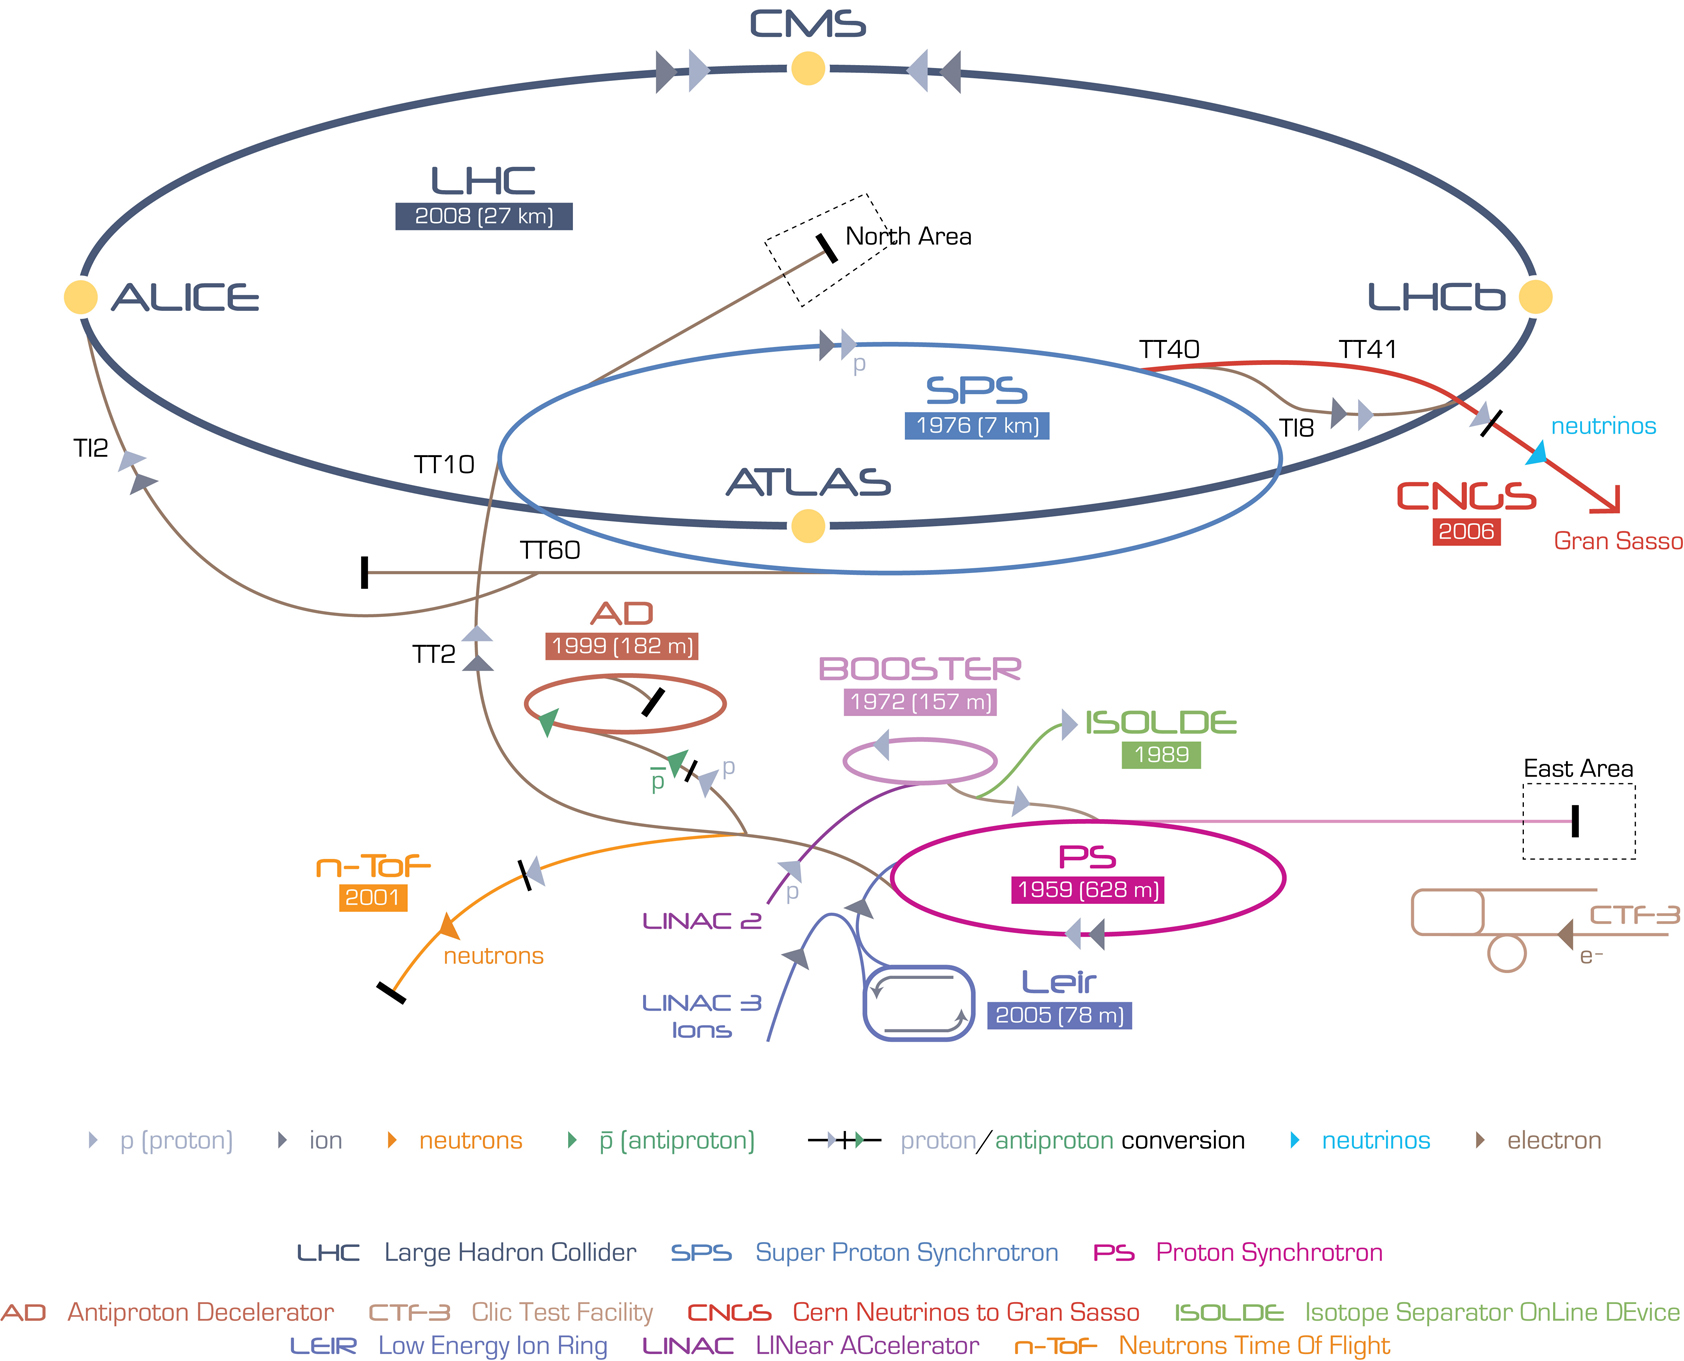
\includegraphics[width=0.65\textwidth]{../figs/Cern-Accelerator-Complex.jpg}
    \caption{Conceptual drawing of all accelerators and experiments hosted at CERN. Besides operating
    the LHC, there are many other accelerators, decelerators and experiments being operated.}
    \label{fig:accelerators}
\end{figure}

Protons used for acceleration in the LHC are extracted from a hydrogen molecules in a bottle situated 
at the CERN main site. These molecules are stripped of their electrons by strong electric fields
and subsequently injected into the first acceleration stage, the linear accelerator Linac 2. Upon exiting
Linac 2, the protons have gained an energy of 50 MeV and are injected into the first circular accelerator,
the Booster. This synchrotron with a circumference of 157 meters accelerates the protons to an energy of 1.4 GeV and
uses magnetic dipole fields to bend the protons onto a circular path. These bending magnets are operated at 
room temperature for the Booster and in fact all the accelerators up to the LHC.
From the Booster, the protons are injected further into the Proton Synchrotron, an accelerator originally built
in 1959 with a circumference of 628 meters and an output energy of 25 GeV. The last step before injection into
the LHC is the Super Proton Synchrotron (SPS), which accelerates the protons to the LHC injection energy of 450 GeV.
The SPS is the world's second largest accelerator with a circumference of nearly 7 km, and it was the first accelerator
to collide protons and anti-protons at energies high enough to produce $W$ and $Z$ bosons, leading to their discovery in 1983
\cite{Wdiscovery, Zdiscovery}.

Ions pass through the same accelerators on their way to the LHC, the only difference being the
first linear accelerator, which in the case of heavy ions is Linac 3.

While the LHC is filled and delivering collisions to its experiments, the accelerators are used to provide
particles to other experiments ongoing at CERN. The Antiproton Decelerator (AD) in which anti-protons are 
decelerated and combined with positrons to form anti-hydrogen, and the ISOLDE collaboration for the study
of many different radioactive ions are just some of the examples of interesting experiments ongoing at CERN.

\subsection{Specifications of the LHC}
\label{sub:lhc}
The LHC itself is located in a tunnel 50-150 meters below ground and has a total circumference of \num{26659} meters.
Particles are injected from the SPS into the LHC into two counter-rotating beams at the aforementioned
injection energy of 450 GeV. 

In order to measure the performance of a particle accelerator such as the LHC, the quantities of instantaneous and integrated
luminosity are the most important figure of merit, as they correspond to the total number of particle collisions
produced in any given collision point. The instantaneous luminosity is defined as

\begin{equation}
    L = \frac{N_b^2 n_b f_{rev} \gamma_r}{4 \pi \epsilon_n \beta^*} F,
\end{equation}
where $N_b$ denotes the number of particles per bunch, $n_b$ the number of bunches, $f_{rev}$ the revolution 
frequency of each bunch, $\gamma_r$ the relativistic gamma factor, $\epsilon_n$ the normalized beam emittance,
$\beta^*$ the $\beta$-function of the beam at the collision point, and $F$ a geometrical factor inversely proportional
to the crossing angle at the interaction point. The beam emittance is defined as the 
volume of the beam in the position-momentum phase space and is thus a measure of the quality of the beam. Emittance itself is 
inversely proportional to the beam momentum and it is therefore necessary to introduce a normalized emittance, which does not change
its value with momentum in order to compare beam quality before and after acceleration. The $\beta$-function describes the
behavior of the transverse beam size as a function of the position in the accelerator, and the value $\beta^*$ is consequently
proportional to the transverse size of the beam at the collision point.

The dimension of the instantaneous luminosity is $cm^{-2}s^{-1}$ and by integrating the instantaneous luminosity over time
the integrated luminosity $\mathfrak{L}_{int}$ can be obtained. Through knowledge of the latter, one can calculate the total number
of expected events for any given physical process in a data sample of a given size by
\begin{equation}
    N_{\text{process}} = \mathfrak{L}_{int} \cdot \sigma_{\text{process}}.
\end{equation}

All relevant beam parameters to calculate the instantaneous luminosity at the LHC are summarized in Table~\ref{tab:lhc}
at both injection and collision energies. It is important to note that these values refer to the design of the LHC and
would result in an instantaneous luminosity of \num{1e34} $cm^{-2}s^{-1}$ at a spacing between the bunches
of 25 ns. However, the actual performance of the machine between first stable operations in 2009 and the first long 
shutdown at the beginning of 2013 has been outstanding. Despite the fact that only half the bunches were filled, resulting in 
a bunch spacing of 50 ns, many beam parameters have already exceeded their design values which lead to a maximum 
instantaneous luminosity of \num{7.67e33} $cm^{-2}s^{-1}$. 




\begin{table}
    \begin{center}
    \caption{Beam parameters for beams in the LHC at injection and collision energy.}
    \label{tab:lhc}
    \begin{tabular}{ r l | c | c }
   & & Injection & Collision \\ \hline \hline
    \multicolumn{4}{c}{\textbf{Beam parameters}} \\ \hline
    Beam Energy & [GeV]   &  450   & 3500 - 7000 \\ \hline
    Relativistic $\gamma_r$ &  &  479.6   & xxxx-7461 \\ \hline
    Particles per bunch & & \multicolumn{2}{c|}{\num{1.15e11}} \\ \hline
    No. of bunches  & &  \multicolumn{2}{c|}{2808} \\ \hline
    $f_{rev}$& [Hz]   & & 11245 \\ \hline
    $\epsilon_n$  & [$\mu$m rad] & 3.5 & 3.75 \\ \hline
    Half crossing angle\footnote{\label{note1}at CMS and ATLAS} &[$\mu$rad] & $\pm$ 160 & $\pm$ 142.5 \\ \hline
    $\beta^*$& [m] & 18 & 0.55 \\ \hline %\footnotemark[\ref{note1}]
%    Beam energy per beam [MJ] & 23.3 & 362 \\ \hline
%    Synchrotron radiation per ring [W]& \num{6.15e-2} & \num{3.6e3} \\ \hline
    \hline
    \end{tabular}
    \end{center}
\end{table}
